Using an identical algorithm, we will now solve a thermal compliance problem
that will be revisited with EFEM in \autoref{sec:thermal_compliance_classic_unit_square};
the algorithm, implementation, and derivation are worked out in greater detail in \autoref{sec:toph_appendix}.

\begin{figure}[ht]
    \centering
    \caption[b]{$\Omega$ for \texttt{toph}.}
    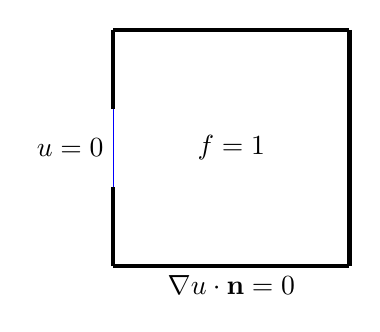
\begin{tikzpicture}
        \draw [ultra thick] (0,0) -- (0,1);
        \draw [blue] (0,1) -- (0,2);
        \draw [ultra thick] (0,2) -- (0,3);
        \draw [ultra thick] (3,3) -- (0,3);
        \draw [ultra thick] (0,0) -- (3,0);
        \draw [ultra thick] (3,3) -- (3,0);

        \node at (0, 1.5) [anchor = east] {$u = 0$};
        \node at (1.5, 1.5) {$f = 1$};
        \node at (1.5, 0) [anchor = north] {$\nabla u \cdot \mathbf{n} = 0$};
    \end{tikzpicture}
\end{figure}

That is, $\Omega$ is a square with a small component of the left side cut out allowing heat to flow through;
the interior of the domain is evenly heated. We again discretize with square elements.

\subsection{Results}

First with a 40x40 square discretization, mass fraction $\theta = 0.4$, SIMP penalization exponent of $3.0$,
and $r_\text{min}$ of 1.2, and secondly with an 80x80 square.

Keeping the constant even heating in mind, the solution reached is fairly natural: the goal
is essentially to a build a heatsink that draws heat from $\Omega$ out to the left. So, the
tree structure formed first serves this purpose as a conductor and secondly maximizes the surface area
(which can be seen as the mesh is refined).
\vfill\pagebreak

\begin{figure}[H]
    \centering
    \caption{40x40 \texttt{toph} simulation.}
    \includegraphics[width=0.8\textwidth]{imgs/TopH/toph_1.png}
\end{figure}

\begin{figure}[H]
    \centering
    \caption{80x80 \texttt{toph} simulation.}
    \includegraphics[width=0.8\textwidth]{imgs/TopH/toph_2.png}
\end{figure}



